\documentclass[11pt]{article}
\usepackage{fullpage,amsthm,amsfonts,amssymb,epsfig,amsmath,times,amsthm,enumitem,mathtools,graphicx}

\newtheorem{theorem}{Theorem}
\newtheorem{claim}[theorem]{Claim}
\DeclarePairedDelimiter{\ceil}{\lceil}{\rceil}
\graphicspath{{graphs/}}

\begin{document}

\begin{center}
{\bf\Large CMPS 102 --- Winter Quarter 2017 --  Homework 3}\\
{\bf Christopher Hsiao - chhsiao@ucsc.edu - 1398305}
\end{center}

\section*{Solution to Problem 1 - Doing Dishes}

Consider a set $S \text{of} n$ computer scientist roommates who would like to determine "who will do the dishes after dinner" for the next $m$ nights. Not all roommates have dinner jat home every night, so let $S_i$ denote the subset of roommates who will have dinner at home on the $i^{th}$ night and let $w_i \leq |S_i|$ be the number of people needed to do the dishes on the $i^{th}$ night (some nights multiple people are needed).

For each roommate $j \in S$ and night $1 \leq i \leq m$, let $Q_i(j) = 0$ if $j$ does not eat at home on the $i^{th}$ night, otherwise let $Q_i(j) = w_i/|S_i|$, i.e., if $j$ eats at home on the $i^{th}$ night. Now, for each roommate $j$, let
\begin{equation}
	R_j = \sum_{i=1}^{m} Q_i(j) .
\end{equation}

Clearly, we can't hope that everyone does dishes exactly $R_j$ nights since, in general, $R_j$ won't even be an integer.

Nevertheless, the computer scientists claim:
\begin{center}
	There exists a dish-washing plan under which\\
	each roommate $j \in S$ does the dishes at most $\ceil[\big]{R_j}$ times.
\end{center}

Prove the claim. That is, be a computer scientist.

\textbf{Hint:} Formulate as a flow problem between roommates and nights and use the Integrality Theorem.

\noindent\rule{17cm}{0.4pt}

% TODO: IMAGE HERE

We will form our graph as shown above. The source node $s$ is connected to all $n$ people, such that there exists an edge between $s$ and all $\{p_1, p_2, p_3, ... p_n\}$

\pagebreak

\section*{Solution to Problem 2 - Fussy Eaters}

You are planning a dinner party for $n$ friends who, naturally, have all sorts of dietary restrictions and allergies. Your plan is to cook some appetizer dishes and some main dishes and portion them so that you end up with $n$ appetizer \textit{portions} and $n$ main \textit{portions}. You email everyone, and for each person $i \in \{1, ... , n\}$ you get back their list $A_i$ of OK-to-eat appetizer dishes and their list $M_i$ of OK-to-eat main dishes.

Design an efficient algorithm that takes as input the number of portions of each dish and the lists $A_i, M_i$, designs a max flow instance, has it solved, and uses the (value of the) maximum flow to decide whether or not it is possible to give each friend an appetizer and a main portion that is OK for them to eat.

\noindent\rule{17cm}{0.4pt}
\subsection*{Appetizers}
We build the following flow network. There is a node $p_i \in \{p_1, ..., p_n\}$ for each person $i$, and a node $a_j \in \{a_1, ..., a_n\}$ for each appetizer $j$. There is an edge $(p_i, a_j)$ of capacity $1$ if appetizer $a_j \in A_i$, where $A_i$ represents the appetizers person $i$ is okay with eating. We then connect a super-source $s$ to every person node $p_i \in \{p_1, ..., p_n\}$ with an edge $(s, p_i)$ of capacity 1. Then, we connect every appetizer node $a_j \in \{a_1, ..., a_n\}$ to a super-sink $t$ with an edge $(t, a_j)$ with capacity 1.

\begin{center}
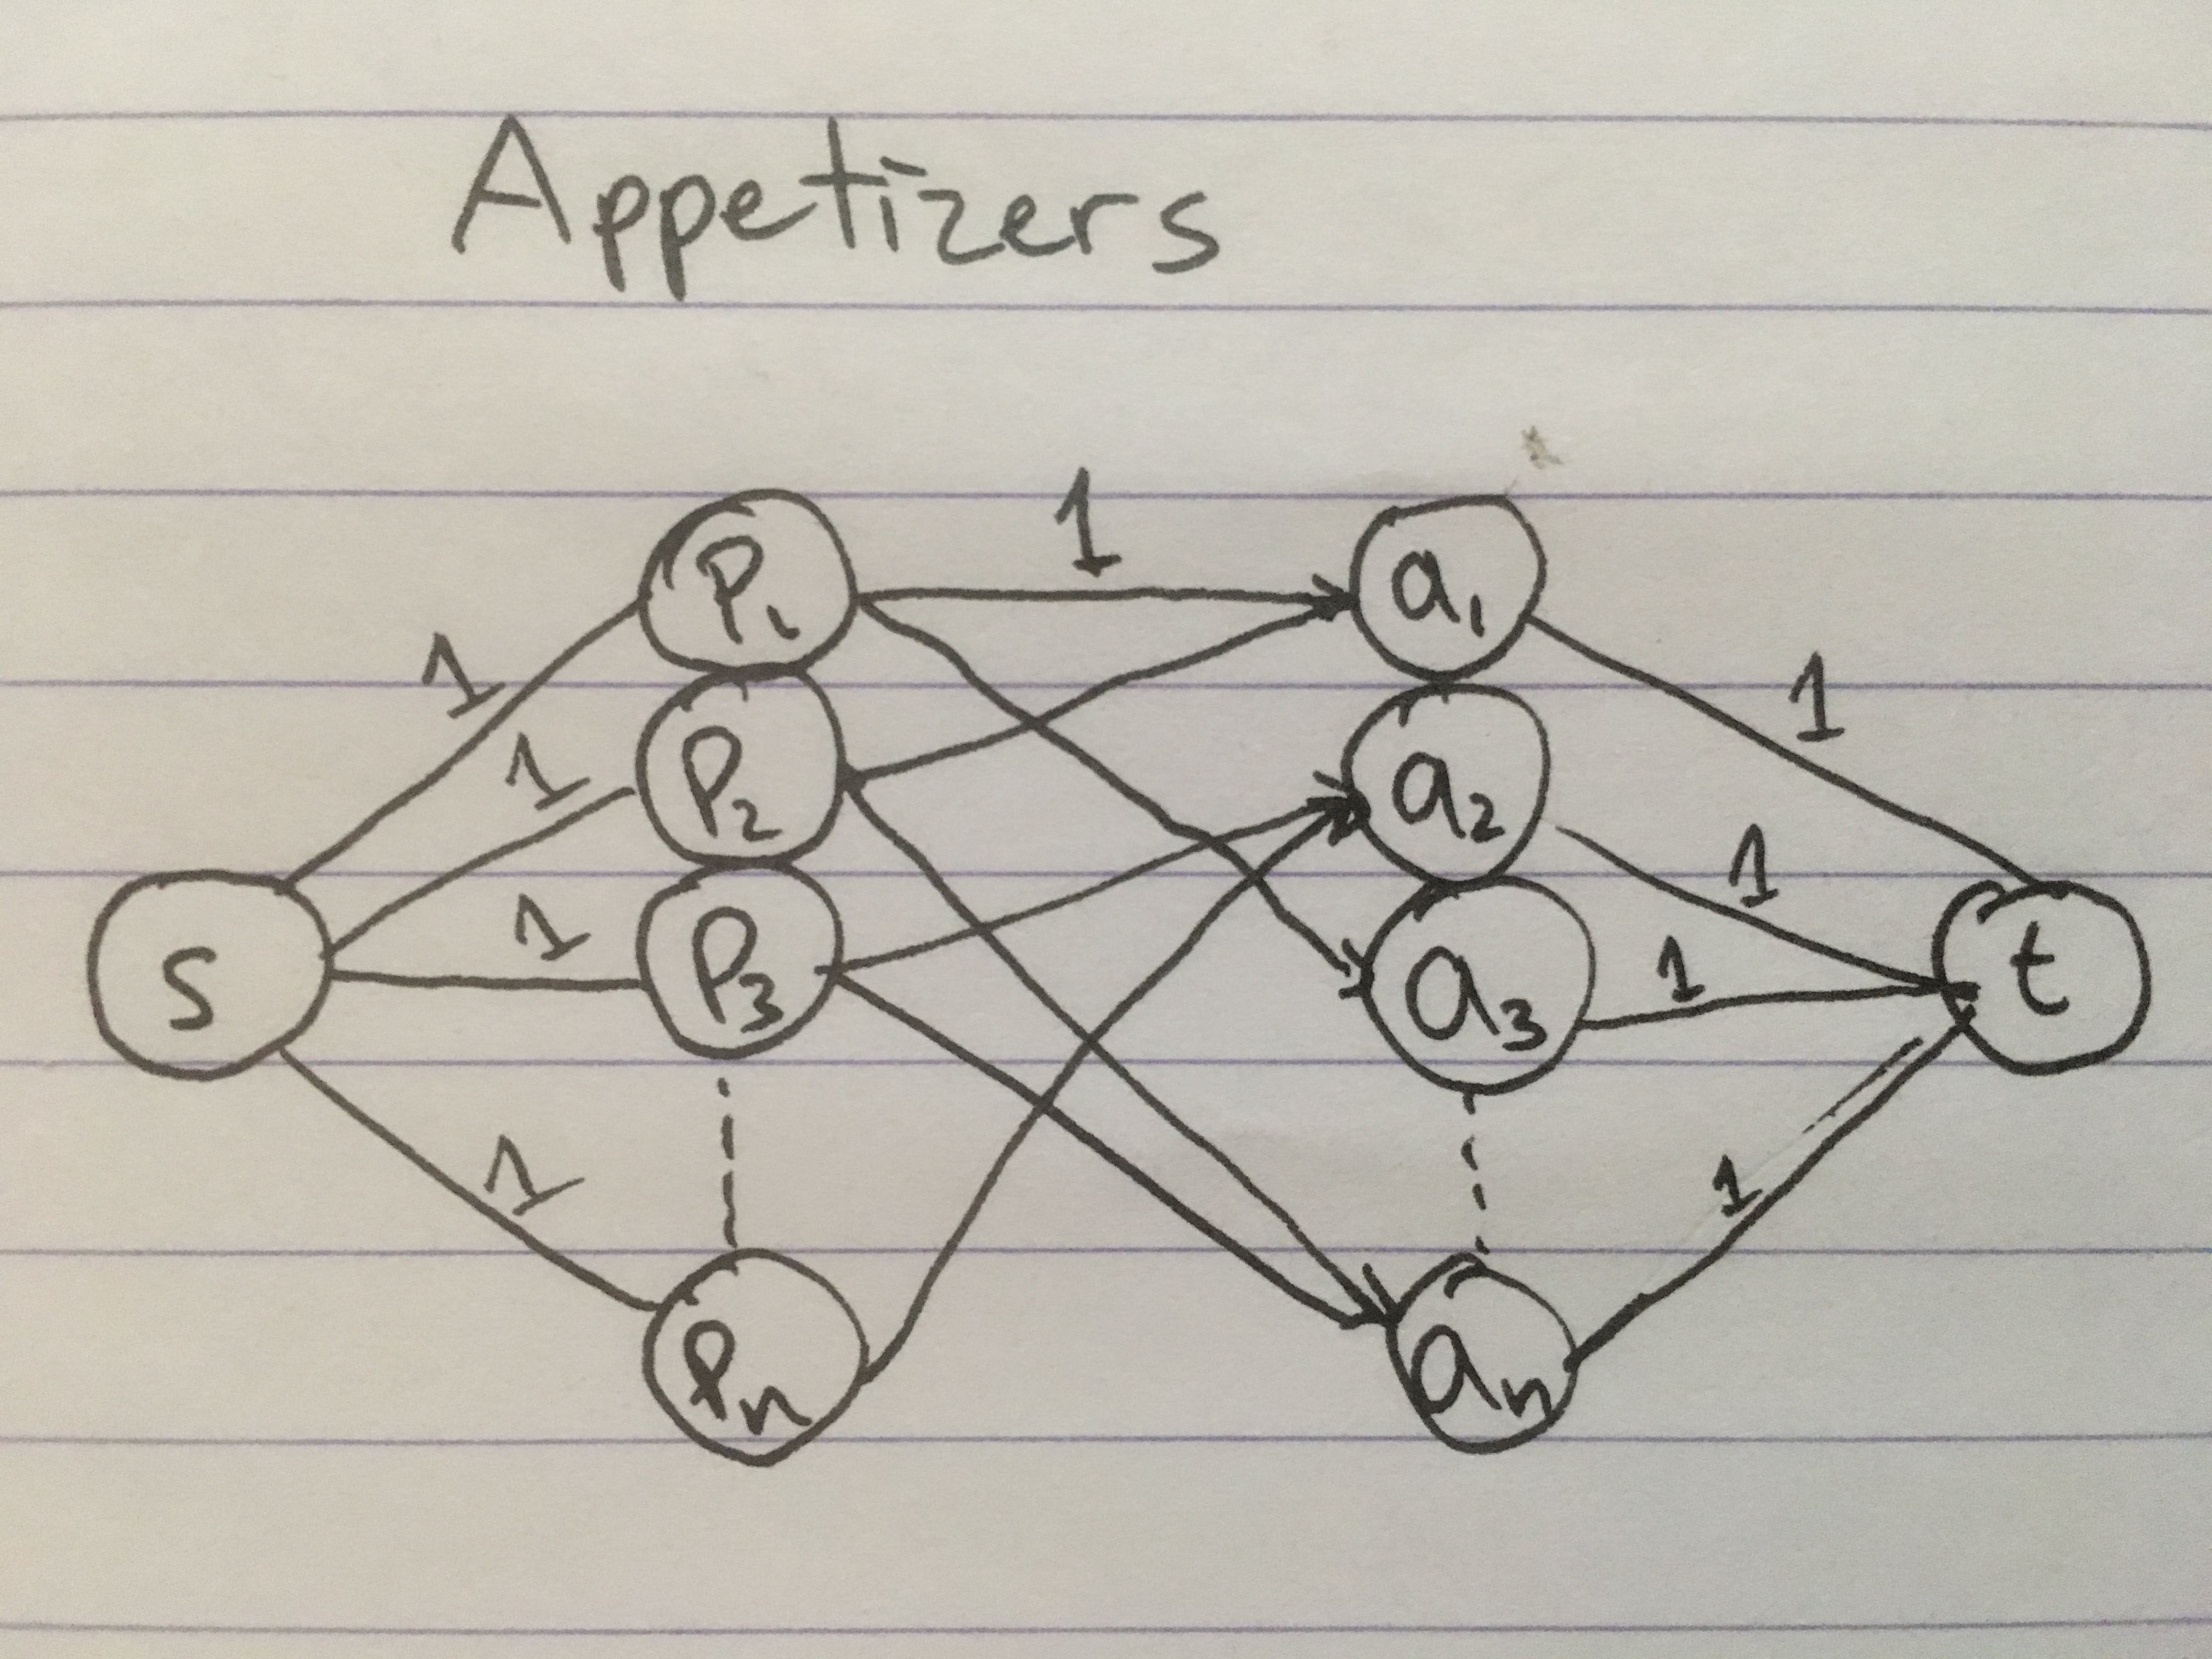
\includegraphics[width=10cm,height=10cm,keepaspectratio]{q2_appetizers}
\end{center}

\begin{claim}
Given a $flow = n$, we can determine an assignment of $n$ people to $n$ dishes such that all people are are satisfied.
\end{claim}

\begin{proof}
There cannot be any $flow > n$, because the total capacity of the cut across the source $s$ leading to the person nodes is $n$. More explicitly, since there are $n$ edges from $s$, each with capacity $1$, there cannot possibly be any flow greater than $n$ across the graph.\\
\\
Now, let us discuss what a max flow of $n$ implies.
\begin{enumerate}
\item All edges $(s, p_i)$ for $i = 1 ... n$ are saturated, as each of the $n$ edges has capacity $1$.
\item All flow was able to traverse the edges $(p_i, a_j)$, such that $n$ flow reaches all $a_j$ nodes.
\item Crucially, there is no "overflow" on any $(a_j, t)$ for $j = 1...n$ edges, as a max flow of $n$ means that all edges directed at $t$ (which have capacity 1) are saturated.
\end{enumerate}

We can find this max flow using $Ford-Fulkerson$. However, note that the flow across the inner edges $(p_i, a_j)$ is distributed, and not necessarily integers. However, by the integrality theorem, since our flow $n$ and all capacities are integral, it then follows that the flow across the inner edges are either $(0, 1)$, with a flow of $1$.
\end{proof}

\begin{claim}
No pairing exists where max flow $< n$ where all guests are satisfied.
\end{claim}
\begin{proof}
From the proof above, we proved that for any flow $f = n$, there exists a stable pairing where no people are dissatisfied. A significant part of the argument was using the saturation of the edges $(a_j, t)$ to represent all appetizers being chosen. For $f < n$, even if the difference $n-f \neq$ some positive integer, it is clear that it is otherwise impossible to saturate some subset of the edges $(a_j, t)$. This means that not all appetizers were able to be "chosen", and some guest was left dissatisfied.. The issue is even more cut and dry when $n-f =$ some integer, because that means only $n-1$ appetizers were chosen, and some guest was left appetizer-less (and dissatisfied). 
\end{proof}

The runtime of this algorithm is simply the runtime of the $Ford-Fulkerson$ algorithm, which runs in $O(\text{people} \cdot \text{appetizers})$. Since there are $n$ people and $n$ appetizers, the runtime therefore is $O(n^2)$.

\subsection*{Main Dishes}

\pagebreak

\section*{Solution to Problem 3 - Verbal Assault}

You are an English teacher assigning presentations to students. Each of your $n$ students will receive a topic and 31 fancy words that they must use in discussing the topic. You've announced the set of topics $T$ and the set of fancy words $F$, and have received from each student $i \in \{1, ..., n\}$ a set $T_i \subseteq T$ of topics the student is interested in, and a set $F_i \subseteq F$ of fancy words that the student would like to use.

You want to see if it is possible to assign to each student a topic and \textit{exactly} 31 words such that:
\begin{itemize}
	\item Each topic is assigned to at most 2 students.
	\item Each fancy word $w_i$ is assigned to at most $t_i$ students.
\end{itemize}

Describe a method that takes as input the sets $T_i$ and $F_i$ and the number $t_1, ..., t_k$ and returns either "No", or an assignment of topics and words that meets the requirements.

\noindent\rule{17cm}{0.4pt}

\pagebreak

\section*{Solution to Problem 4 - Mi-$k$ Drop}

Let $G = (V,E)$ be a directed graph with a source $s \in V$, a sink $t \in V$, and where every edge $e \in E$ has capacity exactly 1. Let $k$ be he value of the maximum flow in $G$.

\textbf{Question:} Given an arbitrary integer $1 \leq q \leq k$, can you always remove $q$ edges from $G$ so that in the resulting graph $G'$ the value of the maximum flow is $k-q$?

\noindent\rule{17cm}{0.4pt}

Yes.

\begin{proof}
By the MaxFlow-MinCut theorem, the maximum flow in a network is bounded by $|min\text{ }cut|$, which means that if $k$ is the maximum flow in $G$, then $k$ is also $|min\text{ }cut|$. Since $|min\text{ }cut|$ acts as an upper bound on our flow, it stands that removing edges in $G$ is a perfectly valid operation as long as the number of edges removed is bounded by $1 \leq q \leq k$. Since every edge in $G$ has capacity $1$, removing any edge  reduces the maximum flow by 1. Repeat this process $q$ times, and you have a max flow reduced by $q$, aka $k-q$.
\end{proof} 

\end{document}
